\documentclass[sigconf]{acmart}

\AtBeginDocument{%
  \providecommand\BibTeX{{%
    \normalfont B\kern-0.5em{\scshape i\kern-0.25em b}\kern-0.8em\TeX}}}

\usepackage{dblfloatfix}
\usepackage[acronym]{glossaries}

\begin{document}

\newacronym{SMART}{SMART}{SeMantic AnsweR Type}
\newacronym{ATP}{ATP}{Answer Type Prediction}
\newacronym{BERT}{BERT}{Bidirectional Encoder Representations from Transformers}

%\title{Semantic Answer Type Prediction 2020}
\title{%
  Semantic Answer Type Prediction 2020 \\
  \large Team-018}

% AUTHORS:
\author{Stephan Frederik Werner Brandasu}
\affiliation{University of Stavanger}
\email{sf.brandasu@stud.uis.no}

% DATE:
\date{\today}



\begin{abstract}
We describe our solution to the \gls{SMART} prediction task 2020 for the DBpedia dataset. Our methods will take advantage of BM25 scores that get modified by the presence of specific keywords in the questions.
\end{abstract}

\keywords{information retrieval, answer category classification, answer type prediction, natural language understanding, understanding query types}

%% Remove copyright footer
\settopmatter{printacmref=false}
\setcopyright{none}
\renewcommand\footnotetextcopyrightpermission[1]{}
\pagestyle{plain}
%% ------------------------

%%
%% This command processes the author and affiliation and title
%% information and builds the first part of the formatted document.
\maketitle



\section{Introduction}
%Explain the context of the problem that you are tackling, including references to relevant literature.
%% shorten some of the sentences. and maybe increase the introduction length.
%% what are we doing, why is it important and why is it hard.
%% clarify its its question answering or question type answering
\gls{ATP} is a challenging problem in the natural language processing field which is an important step to being able to understand natural language queries. Understand the category and type of a given question is an important step in reaching this goal.

The \gls{SMART} task has provided 2 datasets, one using the DBpedia ontology and another using the Wikidata ontology.
Both datasets follow the same structure and will have a question id, a question text in natural language, an answer category and an answer type. They do differ in one sense though, If the category is a 'resource' then the types from the DBpedia dataset are different from the ones in the Wikidata dataset. This has to be taken into account when attempting to classify the questions.

The goal of this paper is to as accurately as possible classify the category and type of a natural language question.



\section{Related Works}
% add some papers from the smart task, only 2 references so far.
% talk about common methods as well 
% change the heading title
\subsection{Question word categories}
A previous submission to the \gls{SMART} task by \citet{Maryland:qwords} from the University of Maryland found that the category of an answer is highly dependent on the question words. They found for example that questions starting with 'Is' or 'Does' always expect a boolean answer and questions starting with 'when' could expect either a number or a date\cite{Maryland:qwords}. A graph showing the most common question words found by this paper can be seen in figure \ref{figure:firstquestionwords}. 

\begin{figure}[h]
    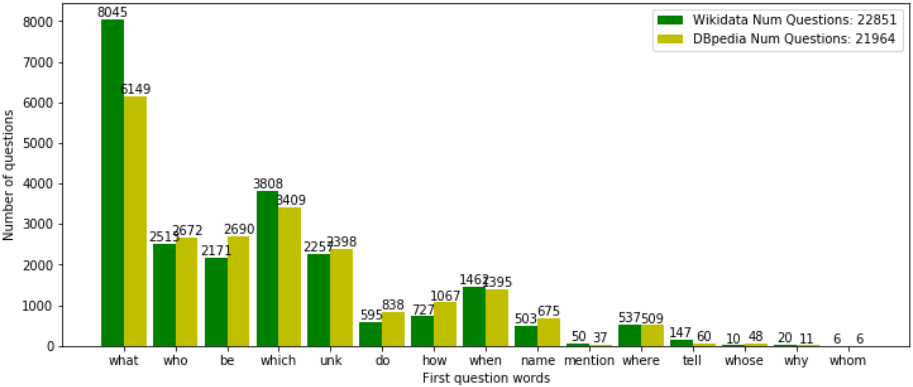
\includegraphics[width=0.48\textwidth]{figures/firstQuestionWords.png}
    \caption{"First words in sentences from Wikidata and DBpedia datasets" by \citet{Maryland:qwords}}
    \label{figure:firstquestionwords}
\end{figure}

\subsection{Most frequent resource types}
The submission by \citet{Kothen:analysis} from the University of Applied Sciences in Kothen Germany did some analysis on the dataset and found that which types of resources came up most commonly over the whole dataset. This information can be used to weigh the possible answers to try to deduce the correct answer type for a given question\cite{Kothen:analysis}. A graph showing the most common answer types found by this paper can be seen in figure \ref{figure:top10resourceanswertypes}.

\begin{figure}[h]
    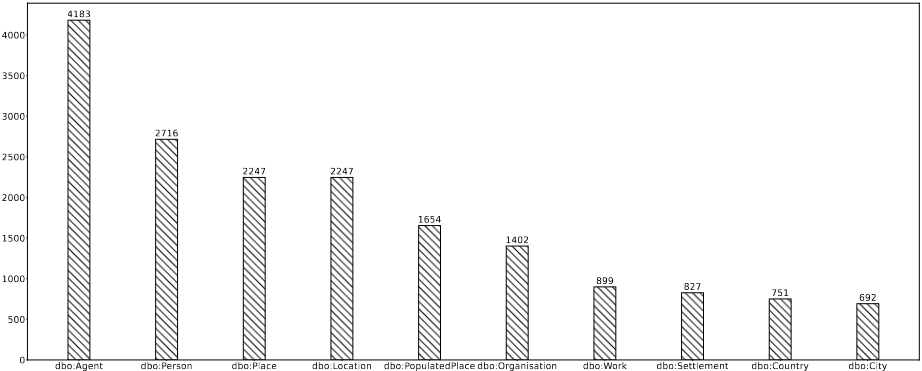
\includegraphics[width=0.48\textwidth]{figures/top10ResourceAnswerTypes.png}
    \caption{"TOP 10 resource answer types" by \citet{Kothen:analysis}}
    \label{figure:top10resourceanswertypes}
\end{figure}

\subsection{Common methods for classification}
A model used frequently used for question classification by previous submissions is \gls{BERT}\cite{maastricht:bert, heraklion:bert, tokyo:bert, uis:bert, Kothen:analysis}. 

\gls{BERT} is an open source machine learning framework used for natural language processing. The model has been pre-trained but also can be fine-tuned with your own datasets. What is unique about BERT is that it can learn bidirectional representations with transformers. This allows for much larger data sets to be analyzed more quickly since words can be processed in relation to all other words at once, instead of one at the time. Additionally by using transformers \gls{BERT} can better understand the context of a word since it compares it to all the other words at once, this makes it extremely capable for text classification tasks such as this.\cite{nvidia:bert}



\section{Problem Statement}
%Formalize the task (in terms of input and output) and specify important details about the data collection.

% problem statement should be a bit longer, talk about datasets that we use. 
% talk about 2 step approach
The objective of this task is to take a natural language question and correctly classify the category and types expected from said question. More broadly this means that a systems needs to be created which takes a normal human written sentence and knows whether to categorise this question as a resource, a literal or as a boolean. Depending on the category it must also identify the correct types for each given category. 

A boolean can only have boolean as a type. Meanwhile a literal could be expecting a string, a date or a number as a type. Resources expect more specific type predictions, first of all if the category is resource then there is a chance more than 1 type is expected as an answer. Second of all the types are expected to exist within a hierarchy based on how specific they are.



%% finish up until here for deadline 1
\section{Baseline Method}
%Explain what you are taking as your baseline method, as well as why this is a reasonable baseline, and why you are making specific implementation choices.
First we must create two different indices for each stage of question classification. The first index is a collection of both the DBpedia and the Wikidata training dataset. These datasets get combined and each question gets preprocessed. The preprocessing simply removes any punctuation and stems the questions using the Porter Stemmer. No stop word removal is done because they could be important to understanding the question. After the preprocessing the questions get indexed using Elasticsearch where their document id will be the training set question id and then the document will have a field containing the question, the category and its types. 

The second index is a collection of descriptions and types belonging to descriptions from a DBpedia data dump. First we take the dump of instances from DBpedia where a page is linked to a type and we 'clean' this list where we will merge entries that have multiple types. Then we will take the dump of abstracts that links a page to a description. This description will get preprocessed like before except this time the preprocessing also removes stop words so that the descriptions should primarily contain key-words. For each description id we check if we there is a match with the same id in the instances list. If there is then we add the corresponding types to the description, if not then we don't index the description. 

\hfill \break
For clarity of which dataset is being talked about going forward. A 'question' is referring to a question from the indexed training datasets. A 'query' is referring to a question from the test dataset which is being classified. 
\hfill \break

Once these indices are in place we can start actually classifying the queries. The first step is to compare the queries to the indexed training dataset. We will use the Elasticsearch \emph{search} function which uses BM25 scoring to create a list of the most relevant questions relative to the query. We simply take the first result from \emph{search} and we use Elasticsearch \emph{get} to retrieve the category and type of the question which best matched the query.

From here we enter the second stage of classification. If the category from the first stage is either 'boolean' or 'literal' we don't do any further classification. If the category is 'resource' then we will clear the existing list of types and replace them in the following way:

In the second stage of classification will only apply if the category is a 'resource'. What is done here is again we will us Elasticsearch \emph{search} to find the best match for the query. But instead of searching the questions from the training datasets we now search the indexed collection of descriptions and types from the DBpedia data dump. The other difference for the second stage is that instead of only taking the top result, we will now try to take the top 20 results. For each result we will again use Elasticsearch \emph{get} to retrieve the types of a document, then we will iterate through each type and add it to the list of types for the query. If the type already exists in the type list then we don't add it to avoid redundancy. We will also stop adding types once the type list has 10 entries in it due to the evaluating only considering up to 10 types. 

\hfill \break

The reason that we first compare the query to the training questions and then to the DBpedia data dump is to try to prioritise getting the "easier" categories where there are only 1 or 3 possible types correct. Doing the category prediction first using the training datasets seemed like the most intuitive way of achieving this. 

Then for the second stage, the reason we go through up to 20 results from the DBpedia data dump, even though we only want to take 10 types from the results, is that it was chosen to try to prioritise getting a better $NDCG@10$ score by trying to make sure that the classification will try to "guess" as many types as possible. Depending on the amount of results we won't necessarily get 10 types but we always try to get this many to give as many "relevant enough" types as possible. 

\begin{table}[h]
    \centering
    \caption{Baseline method results}
    \begin{tabular}{c|c|c}
    $Accuracy$ & $NDCG@5$ & $NDCG@10$ \\
    \hline
    0.916 & 0.487 & 0.489
    \end{tabular}
    \label{tab:baseline_res}
\end{table}

We can see the results for the baseline methods in table \ref{tab:baseline_res}. Here we can see that the category prediction is correct a large majority of the time. The type prediction meanwhile performs worse and differently depending on how many types we consider. The results are slightly better when we look at the score for 10 types instead of 5, this makes sense considering the focus on "guessing" as many types as possible.

% finish up until here for deadline 2
\section{Advanced Method}
%Explain what you are taking as your advanced method(s), as well as why this is a promising attempt to outperform the baseline method, and why you are making specific implementation choices.
For the advanced method we make some changes to the category and type prediction in an attempt to fine tune the results. First of all in the category prediction, before we search the indexed collection of questions, we check if the query contains the words 'how many' after each other. The chance that somebody is asking 'how many x' and isn't expecting a number as a response was decided to be almost 0. So these 2 words coming after each other will always return 'literal' as the category and 'number' as the type. 

Additionally during the category prediction we will now attempt to re-weigh the scoring by looking at the first word of the question. First the initial \emph{search} will take the top 10 results instead of only the top result. For each of these results we will save the top result from each category if it exists. From there for each top result for a given category we will increase the score based on the first word in the query. 

The score increases were decided by analysing the training dataset and first finding the words that would most commonly appear at the start of sentences. Then we would check each word to see how often it appears in a given category. For example we found that when the first word is 'give' it is a 'resource' 66\% of the time and a 'literal' 33\% of the time. These values would be used for the score increases. So if a word was a resource 66\% of the time we would increase the score by $6.6$. The minimum score increase is 0.1 if it appears 1\% of the time and 10 if it was 100\% of the time. 

\begin{table}[h]
    \centering
    \caption{Advanced method results}
    \begin{tabular}{c|c|c}
    $Accuracy$ & $NDCG@5$ & $NDCG@10$ \\
    \hline
    0.940 & 0.524 & 0.538
    \end{tabular}
    \label{tab:baseline_res}
\end{table}


\section{Results}
%With tables and graphs, make a clear, concise, and digestible presentation of the data produced by your experiments. This includes describing the key facts and trend from your results.


\begin{table}[h]
\begin{center}
\caption{Summary of results}
\begin{tabular}{l|c|c|c}
     & $Accuracy$ & $NDCG@5$ & $NDCG@10$ \\
    \hline
    Baseline & 0.916 &  0.487 & 0.489 \\
    Advanced Method & 0.940 & 0.524 &  0.538 \\
\end{tabular}
\label{table:1}
\end{center}
\end{table}



\section{Discussion and Conclusions}
%Summarize and discuss different challenges you faced and how you solved those. Include interpretations of the key facts and trends you observed and pointed out in the Results section. Which method performed best, and why? Speculate: What could you have done differently, and what consequences would that have had?



%%
%% If your work has an appendix, this is the place to put it.
%\appendix

%\section{Appendix}


%%
%% The next two lines define the bibliography style to be used, and
%% the bibliography file.
\bibliographystyle{ACM-Reference-Format}
\bibliography{base}

\newpage
\appendix
\section{GitHub}
The project code and datasets can be found here:

\href{https://github.com/sbthepotato/DAT640-Project-22H}{github.com/sbthepotato/DAT640-Project-22H}

\section{Division of Work During the Project}

The whole project was completed by me so this is not relevant.
% remember to keep this up to date
%\begin{center}
%\begin{tabular}{c|c|c|c} 
% week/name & Evans & Peter & Stephan \\ 
% \hline
% 39 & 0 & 0 & 4 \\ 
% 40 & 0 & 0 & 6 \\ 
% 41 & 0 & 0 & 4 \\
% 42 & 0 & 0 & 10 \\
% 43 & 0 & 0 & 12 \\
% 44 & 0 & 0 & 0 \\
% 45 & 0 & 0 & 0 \\
% 46 & 0 & 0 & 0 \\
%\end{tabular}
%\end{center}


\end{document}
\endinput
